\documentclass{article}
\usepackage{amsmath,amsfonts,amssymb,amsthm}
\usepackage[paperwidth=8.5in,paperheight=10.5 in]{geometry}
\usepackage{color}
\usepackage[bookmarks=false]{hyperref}
\definecolor{myurlcolor}{rgb}{0.8,0,0}
\hypersetup{colorlinks,
linkcolor=myurlcolor,
citecolor=myurlcolor,
urlcolor=myurlcolor}

%Evan's Packages
\usepackage{graphicx}

\newcommand{\define}[1]{{\bf{\boldmath{#1}}}}

\newtheorem{thm}{Theorem}    
\newtheorem{cor}[thm]{Corollary}
\newtheorem{lem}[thm]{Lemma}
\newtheorem{prop}[thm]{Proposition}

\theoremstyle{definition}
\newtheorem{rem}[thm]{Remark}
\newtheorem{defn}[thm]{Definition}
\newtheorem{example}[thm]{Example}

        \newcommand{\be}{\begin{equation}}
        \newcommand{\ee}{\end{equation}}
        \newcommand{\ba}{\begin{eqnarray}}
        \newcommand{\ea}{\end{eqnarray}}
        \newcommand{\ban}{\begin{eqnarray*}}
        \newcommand{\ean}{\end{eqnarray*}}
        \newcommand{\barr}{\begin{array}}
        \newcommand{\earr}{\end{array}}

%maps and arrows
\newcommand{\im}{{\rm im}}
\renewcommand{\hom}{{\rm hom}}
\newcommand{\To}{\Rightarrow}
\renewcommand{\to}{\rightarrow}
\newcommand{\tensor}{\otimes}
\newcommand{\maps}{\colon}

%miscellaneous junk
\newcommand{\id}{{\rm id}}
\newcommand{\op}{{\rm op}}
\newcommand{\iso}{\cong}
\newcommand{\R}{{\mathbb R}}
\newcommand{\C}{{\mathbb C}}
\newcommand{\F}{{\mathbb F}}
\newcommand{\N}{{\mathbb N}}
\newcommand{\Q}{{\mathbb Q}}
\newcommand{\Z}{{\mathbb Z}}
\newcommand{\A}{{\mathcal A}}
\newcommand{\E}{{\mathcal E}}
\renewcommand{\P}{{\mathcal P}}
\newcommand{\M}{{\mathcal M}}
\newcommand{\NN}{{\mathcal N}}
\newcommand{\B}{{\mathcal B}}

\pagestyle{empty}
\pagenumbering{none}

\graphicspath{{images/}}
\begin{document}
\noindent Evan Wilbur \\
CS14 Winter 2016\\
\begin{center}
Lab 2 Report
\end{center}

The program implements all three varieties within their own distinct class, each deriving from an abstract base class, Martian. While the abstract class is not necessary, it was useful to use as it allowed and provided a greater coherency between the  different implementations. Namely, many of the functions found within the abstract base are found frequently throughout the derived classes. There are three derived classes in total representing the three implementations. Two of them, Smart and Dumb, derive Martian directly while Cache derives from Smart as it runs Smart's algorithms provided the table lookup fails.\\
\\
\indent The Dumb class certainly lives up to its namesake. It was purposely designed to be as inefficient as possible. When solving, the program loops through every square number less than the value, subtracts it, then recursively solves what remains. Each instance of a new class increases the tick count by one. The only time saving measure taken is that it checks to see if the number is a perfect square first. Despite this, the program unsurprisingly has a time complexity of $O(2^x)$. This can be easily seen from the graph below. One can also reason that increasing the value $n$ to solve effectively doubles the number of recursive calls one must do. Indeed, when solving for $n+1$, the program will also solve for $n$. Because the steps to solve for $n$ are essentially the same number as the steps for $n+1$ without the recursive call, the number of ticks doubles as the value of $n$ increases.
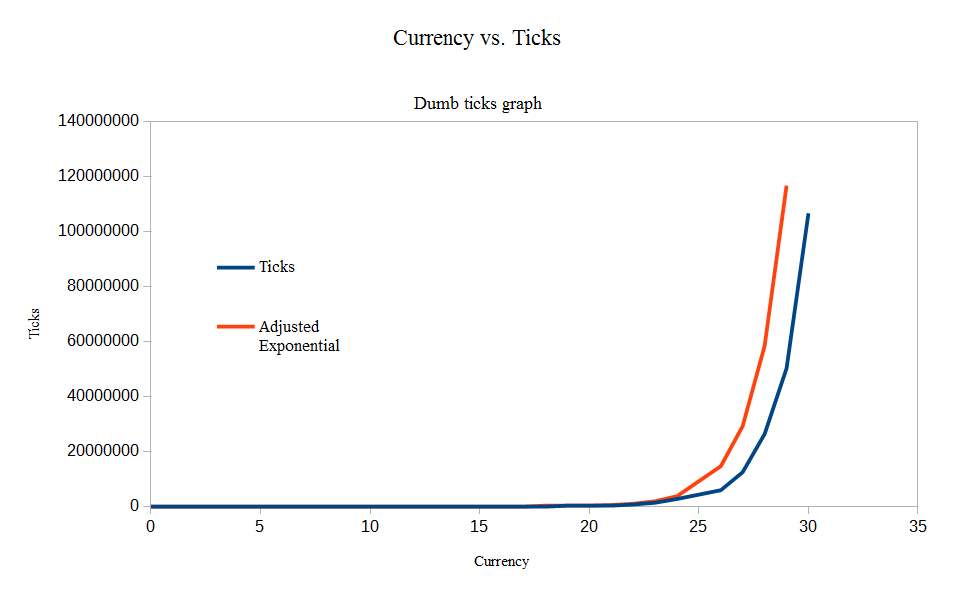
\includegraphics[width=\linewidth]{Dumb_reg}
\\
\indent Cache and Smart are similar as Cache derives many parts from Smart. The only real difference between the two is that Cache will first do a table lookup to see if a solution has already been found. Smart works by implementing Lagrandre's and Legrendre's Theorems'. With them the program can very quickly determine the type of solution present and adjust accordingly. This turns out to be very efficient and it requires very little guessing. Based of the results from the graph it seems apparent that the time complexity of both is $O(\sqrt{n})$ although I am unable to determine exactly why this is. This value for the complexity came from a simple guess and check approach. While they both grow with the complexity of $O(\sqrt{n})$, it should be important to note that these values are taken in the worst case. The average complexity for Cache and Smart are much lower. 
\begin{center}
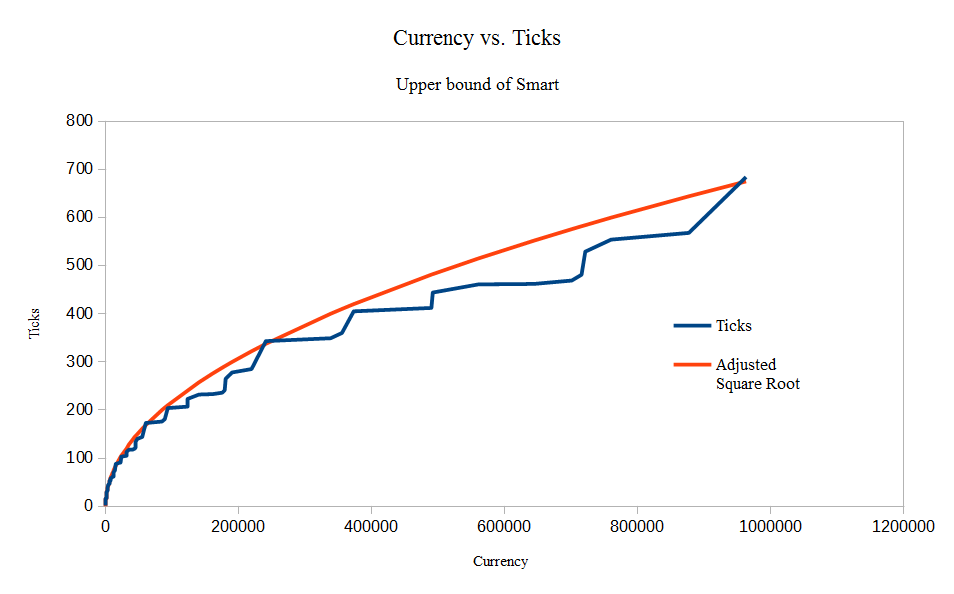
\includegraphics[width=333px]{smart_mil_upper}
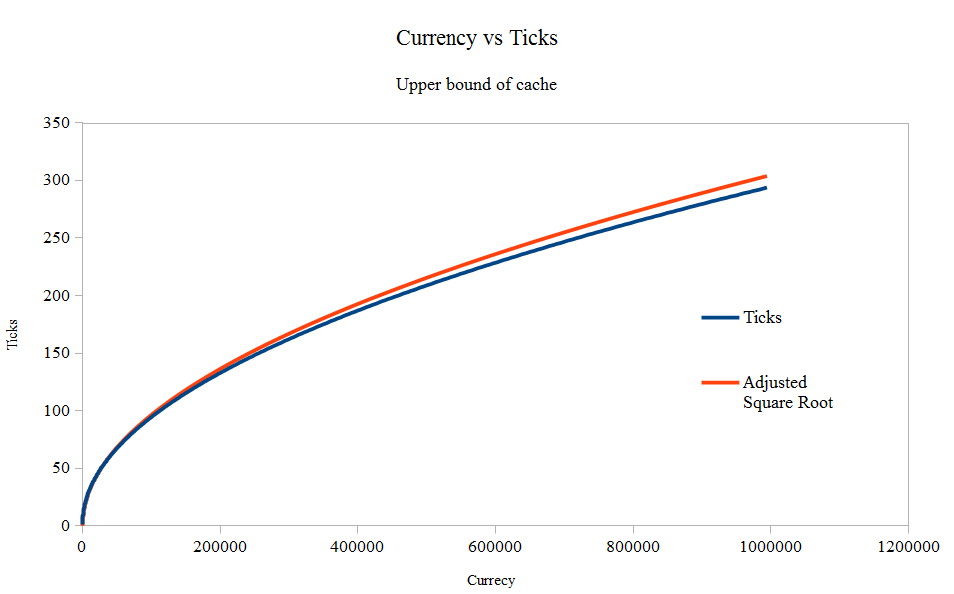
\includegraphics[width=333px]{cache_mil_upper}
\end{center}



\end{document}